\chapter{Geometric Interest Rate Theory}
\section{The Problem}
Any acceptable model which prices interest rate derivatives must fit
the observed term structure. This idea pioneered by Ho and Lee
\cite{HL:1986}, has been explored  in the past by many other
researchers like Black and Karasinski \cite{BK:1991} and Hull and
White \cite{HW:1990}.	 
 
The contemporary models are more complex because they consider the
evolution of the whole forward curve as an infinite system of
stochastic differential equations (Heath, 
Jarrow and Morton \cite{HJM:1992}). In particular, they use 
a continuous forward rate curve as initial input. In reality, one only
observes a discrete set composed either by bond prices or swap
rates. So, in practice, the usual approach is to interpolate the
forward curve by using splines or other parametrized families of
functions. 

A very plausible question arises at this point: Choose a specific parametric
family, $\mathcal{G}$, of functions that represent the forward curve,
and also an arbitrage free interest rate model $\mathcal{M}$. Assume
that we use an initial 
curve that lay within as input for model $\mathcal{M}$. Will this interest rate
model evolve through forward curves that lay within the family?
Motivated by this question, Bj\"ork and Christensen \cite{BC:1999}
define the so--called consistent pairs ($\mathcal{M}$, $\mathcal{G}$)
as ones whose answer to the above  
question is positive. In particular, they studied the
problem of consistency between the family of curves proposed by Nelson
and Siegel \cite{NS:1987} and any HJM interest rate model with
deterministic volatility, obtaining that there is no such interest
model consistent with it. 

We remark that the Nelson and Siegel interpolating scheme 
is an important example of a parametric
family of forward curves, because it is widely adopted by central banks (see for
instance BIS \cite{BIS:2005}). Its forward curve shape,
$G_{NS}(\boldmath{z},\cdot)$ is given by   
the expression
$$
G_{NS}(z,x)=z_1+z_2 e^{-z_4 x}+z_3 x e^{-z_4 x},
$$
where $x$ denotes time to maturity and $z$ the parameter vector 
$$
z=[z_1\;z_2\;\dots]^T.  
$$
Despite all the positive empirical features and
general acceptance by the financial community, Filipovi\`c \cite{Fil:1999} has
shown that there is no It\^o process that is consistent with the
Nelson-Siegel family.     
In a recent study De Rossi \cite{R:2004} applies consistency results
to propose a consistent exponential dynamic model, and estimates it 
using data on LIBOR and UK swap rates. On the other hand, Buraschi and Corielli
\cite{BCo:2005} add results to theoretical framework indicating that the use of
inconsistent parametric families to obtain smooth interest rate curves, 
violates the standard self financing arguments of replicating strategies,
with direct consequences in risk management procedures.

In order to illustrate this situation, we describe a very common fixed-income market
procedure. In the real world, practitioners usually re-estimate yield
curve and HJM model parameters on a daily basis. This procedure
consists of two steps:  
\begin{itemize}
\item They fit the initial yield curve from discrete market data (bond prices,
  swap rates, short-term zero rates), and
\item They obtain an estimate of the parameters of the HJM model, minimizing
  the pricing error of some actively traded (plain vanilla) interest rate
  derivatives (commonly swap options or caps).
\end{itemize}
In contrast with the parsimonious assumption that model parameters are
constant, an unstable HJM model parameter estimation it is often
observed. Perhaps, this 
fact is not relevant for mark to market, but it could have practical 
consequences on the hedging portfolios associated with these financial
instruments. Recall that  
such dynamic strategies depend on the model assumptions. Thus,
re-calibration is conceivable 
because the practitioners are aware of {\sl model risk}. A particular
HJM model is not a perfect description of reality, and they are forced
to re-estimate day to day model parameters in order to include new
information that arrives from the market.  
On the other hand, unstable estimates may be caused by reasons that
are more theoretical, 
because the above mentioned set-up does not take into account that HJM model
parameters are linked, in general, to the initial yield curve fit
parameters. If a practitioner uses an interpolation scheme which is
not consistent with the model, then the parameters will be
artificially forced to change. 
Thus, it seems to be that there are a plethora of motivations for the
study of the empirical evidence and the practical implications that
are predicted by a consistent HJM build model.  

% The consistency hypothesis stated by Bj\"ork, implies that the zero
% coupon bond curve has to be determined at the same time as the
% parameters of the model.

\section{Setup}
We consider, as earlier in chapter 2, a given forward rate model under a
risk neutral martingale measure $\mathbb{Q}$. We will adopt the
Musiela parameterization \cite{Mu:1993} and use the notation 
$$
f(t,x):=F(t,t+x).
$$
The reasons why this parameterization is better suited to address the
main problems that are the subject of the present work have been
accurately explained, for instance, by Filipovi\`c
\cite{Fil:2001}. As we will see, this parametrization makes changes in
the specification of the stochastic process originally proposed by HJM
for the instantaneous forward rate process, $F(t,t+x)$, since now $x$
is not considered any more a fixed variable which parametrizes the
dynamics of these rates. 
\begin{propos}[The Musiela HJM formulation.] Under the martingale
  measure $\mathbb{Q}$ the $f$-dynamics are given by
\begin{equation}
\label{HJMM:2}
\left\{
\begin{array}{rcl}
df(t,x)& = & \left( \frac{\partial f(t,x)}{\partial x}+
  \widetilde\sigma(t,x)\displaystyle \int_0^x \widetilde\sigma(t,u)^T
  \,du\right) dt + \widetilde\sigma(t,x)dW (t) \\  
f(0,x) & = & f^o(0,x).
\end{array}
\right.
\end{equation}
where $\widetilde \sigma(t,x):=\sigma(t,t+x)$.
\end{propos}
\begin{demo}
See Appendix B. 
\end{demo} 

From now, with a clear abuse of notation we remove the symbol
$\;\widetilde{}\;$ from $\sigma$ because in the whole chapter we will
consider the HJM model under the Musiela parametrization. Thus the
interest rate model $\mathcal{M}$ will be characterized by the
particular volatility function $\sigma(t,x)$ used in the following
$f$-dynamics:
\begin{equation}
\label{HJMM:3}
\begin{array}{rcl}
df(t,x)& = & \left( \partial_x f(t,x)+
  \sigma(t,x)\displaystyle \int_0^x \sigma(t,u)^T
  \,du\right) dt + \sigma(t,x)dW (t).
\end{array}
\end{equation}
\section{The Formalized Problem}
\subsection{The Forward Curve Manifold}
Assume that we have a parametrized family of forward rate curves 
\begin{equation}
\label{ForwardMap}
G: \mathcal{Z} \longrightarrow \mathcal{H},
\end{equation}
with $\mathcal{Z} \subseteq \mathbb{R}^d$ the parameter space. For
each parameter value $z \in \mathcal{Z}$ we have a smooth curve
$G(z)$. The value of this curve at the point $x \in \mathbb{R}_+$ will
be written as $G(z,x)$, so we see that $G$ can also be viewed as the
mapping 
\begin{equation}
\label{ForwardMap2}
G: \mathcal{Z}\times \mathbb{R}_+ \longrightarrow \mathbb{R}.
\end{equation}
The main problem is to determine under which conditions the
$f$-dynamics given by (\ref{HJMM:3}) is {\sl consistent} with the
parametrized family of forward rate curves (\ref{ForwardMap}) as
follows: 
\begin{itemize}
\item Assume that, at an arbitrarily chosen time $t=s$, we have fitted
  a forward curve $G$ to market data, i.e. for some $z^o \in
  \mathcal{Z}$ we have 
$$
f^o(s,s+x)=G(z^o,x), \quad \forall x \geq 0\; ,
$$
\item the {\sl future} forward curves produced by the interest rate
  model (\ref{HJMM:3}) always stay within the given forward curve
  family? In other words, does there exist at every fixed time $t\geq
  s$ some $z\in \mathcal{Z}$ such that
$$
f(t,t+x)=G(z,x), \quad \forall x \geq 0\; ?
$$
\end{itemize}

First, to see more clearly what is going on in differential geometric
terms, we define the {\sl forward curve manifold} $\mathcal{G}$, as
the set of all forward curves produced by the parametrized family. 
\begin{defn} The {\bf forward curve manifold} $\mathcal {G}\subseteq
  \mathcal{H}$ is defined as
$$
\mathcal{G} = Im (G).
$$
\end{defn}
We now move on to give precise mathematical definition of the
consistency property discussed above.
\begin{defn}[Invariant manifold.]
Take as given the $f$-dynamics (\ref{HJMM:3}). Consider also the
forward curve manifold $\mathcal{G}$. We say that $\mathcal{G}$ is
invariant under the action of $f$ if, for each point $(s,f)\in R_+
\times \mathcal{G}$, the condition $f_s \in \mathcal{G}$ implies that
$f_t \in \mathcal{G}$ on a time interval $t-s >0$. 
\end{defn}
The purpose of the following section will be to characterize
invariance in terms of local characteristics of both $\mathcal{G}$ and
$\mathcal{M}$. 
\subsection{The Space}
As the space of forward rate curves we will use a weighted Sobolev
space where a generic point will be denoted by $f$.
\begin{defn}
Consider a fixed real number $\gamma > 0$. The space
$\mathcal{H}_\gamma$ is defined as the space of all differentiable (in
the distributional sense) functions 
$$
f: \mathbb{R}_+ \longrightarrow \mathbb{R}
$$
satisfying the norm condition $\| f \|_\gamma < \infty$. Here the norm
is defined as 
$$
\|f\|^2_\gamma= \int_0^\infty f^2(x) e^{-\gamma x}\; dx+\int_0^\infty
\left(\frac{df}{dx}(x)\right)^2e^{-\gamma  x}\; dx 
$$
\end{defn}
Intuitively, as a specific Sobolev space, $\mathcal{H}_\gamma$ is a
vector space of functions equipped with a norm that is a combination
of $L^2$-norms of the function itself as well as its first
derivative. Recall that $x$ is the time to maturity, as defined in
Sect. 1.1. 

In fact, if we introduce the inner product
$$
(f,g)= \int_0^\infty f(x)g(x) e^{-\gamma x}\; dx+\int_0^\infty
\left(\frac{df}{dx}(x)\right)\left(\frac{dg}{dx}(x)\right) e^{-\gamma
  x}\; dx,
$$
the space $\mathcal{H}_\gamma$ becomes a Hilbert space as proved by
Bj\"ork and Landen \cite{BL:2002}.    
\subsection{The Interest Rate Model}
Finally, let us consider as given a volatility function $\sigma$ of
the form 
$$
\sigma: \mathcal{H}_\gamma \times \mathbb{R}_+ \rightarrow \mathbb{R}^q.
$$
$\sigma(f,x)$ is thus a functional of the infinite dimensional
$f$-variable, and a function of the real variable $x$. Denoting the
forward curve at time $t$ by $f_t$ we then have the following forward
rate equation.
\begin{equation}
\label{GeomHJMM}
df_t(x)=\left\{\frac{\partial}{\partial
    x}f_t(x)+\sigma(f_t,x)\int_0^x \sigma(f_t,u)^T\; du \right\} dt+ 
\sigma(f_t,x)\; dW_t.
\end{equation}
\section{The Invariance Conditions}
As we see before, the pair ($\mathcal{M}$, $\mathcal{G}$) is
consistent if and only if the forward curve manifold $\mathcal{G}$ is
invariant under the action $f$, and the question we pursue from now is
when it happens. In order to guess the precise answer we have to
rewrite the analysis in terms of Stratonovich integrals instead of
It\^o integrals.
\begin{defn}
For given semimartingales $X$ and $Y$ driven by a multidimensional
Wiener process, the {\bf Stratonovich integral} of $X$ w.r.t $Y$,  
$$
\int_0^t X_s \circ dY(s)\;,
$$ 
is defined as
$$
\int_0^t X_s \circ dY_s :=\int_0^t X_s \cdot dY_s+\frac{1}{2} dX_t
\cdot dY_t
$$
\end{defn}
\begin{rmk} For computing the ``quadratic variation process'' $dX_t
  \cdot dY_t$ the usual ``multiplication rules'' $dW \cdot dt=dt \cdot
  dt$, $dW\cdot dW=dt$ must be applied.
\end{rmk}
\begin{propos}[Chain rule.] Assume that the function $F(t,y)$ is
  smooth. Then we have
$$
dF(t,Y_t)=\frac{\partial F }{\partial t}(t,Y_t) dt+\frac{\partial F
}{\partial y}(t,Y_t) \circ dY_t.
$$
\end{propos}
Note that under the Stratonovich formulation of the stochastic
integral, the It\^o formula takes the form of the standard chain rule
of ordinary calculus. Now, returning to the above $f$-dynamics
(\ref{GeomHJMM}), we can write it in terms of Stratonovich calculus as
the following 
\begin{equation}
\label{GeomHJMMStrat}
df_t(x)=\left\{\frac{\partial}{\partial
    x}f_t(x)+\sigma(f_t,x)\int_0^x \sigma(f_t,u)^T\; du \right\} dt -
\frac{1}{2} d\sigma(f_t,x) \cdot dW_t +\sigma(f_t,x) \circ dW_t\;,
\end{equation}
and, as it can be seen, it appears a {\sl quadratic variation term}
commonly known as the {\sl Stratonovich correction}. Note that $\sigma$ is
not a function but a functional, however in practical terms we can
work with the ordinary It\^o formula which is still correct as in the
finite dimensional case. Then,  
\begin{equation}
\begin{array}{rcl}
d \sigma \cdot dW(t)&=&\left(\{ \dots\}dt+\sigma_f'(f_t) \sigma(f_t)^T
  dW_t\right)\cdot dW_t\\
&=& \sigma_f'(f_t) \sigma(f_t)^T dt.
\end{array}
\end{equation}
where $\sigma_f'$ denotes the Frechet derivative of $\sigma$ w.r.t the
$f$-variable. This derivative extends the concept of Jacobian matrix
to the infinite dimensional case. Its formal definition, which is
somewhat technical, is left out. See \cite{PZ:1992}.

Finally, we may write the Stratonovich formulation of the Musiela
equation 
(\ref{GeomHJMMStrat}) as \begin{equation}
\label{GeomHJMStratSimple}
df_t=\mu(f_t)+\sigma(f_t)\circ dW_t
\end{equation}
where
\begin{equation}
\label{DriftGeomHJMStratSimple}
\mu(f_t,x)=\partial_x f_t(x)+ \sigma(f_t,x)\int_0^x \sigma(f_t,u)^T\;
du-\frac{1}{2} \left[\sigma_f'(f_t)\sigma_f(f_t)^T \right](x).
\end{equation}
Let us consider as given the forward curve manifold $\mathcal{G}$: the
relevant concept is the following.
\begin{defn}
Consider a given interest rate model $\mathcal{M}$, specifying a
forward rate process $f_t(x)$, as well as a forward curve manifold
$\mathcal{G}$. We say that $\mathcal{G}$ is $f$-invariant under the
action of the forward rate process $f_t(x)$ if there exists a
stochastic process $Z(t)$ with state space $\mathcal{Z}$ and
possessing a  differential of the form
\begin{equation}
\label{FDR}
dZ(t)=\gamma(t, Z(t))dt + \psi(t, Z(t))\circ dW_t,
\end{equation}
such that, for every fixed choice of initial time s, whenever
$y_s(\cdot)\in\mathcal{G}$, the stochastic process defined by
\begin{equation}
\label{pepe}
y_t(x)=G(Z(t), x),\; \forall t \geq s, \; x\geq 0,
\end{equation}
solves the SDE (\ref{GeomHJMMStrat}) with initial condition
$f_s(\cdot)=y_s(\cdot)$.
\end{defn}
In fact, the stochastic $Z$-process is describing how evolves the
vector parameter $z$ as the forward rate curve moves on the manifold
$\mathcal{G}$. 

We assume that the forward rate It\^o dynamics of $\mathcal{M}$ are
given by (\ref{GeomHJMM}), and that the quadratic variation process
may be written in intensity form:
$$
-\frac{1}{2}\left[\sigma'_f(f_t) \sigma(f_t)^T \right](x) dt= \phi(t,x) dt 
$$
Now we can state and prove the main invariance result.
\begin{tma}[Consistency Conditions.] The forward curve manifold
  $\mathcal{G}$ is $f$ invariant for the forward rate process $f(t,x)$
  in $\mathcal{M}$ iff
\begin{equation}
\label{CDC}
G_x(z, \cdot)+\sigma(t,\cdot) \displaystyle \int_0^\cdot \sigma(t,u)^T
\; du+\phi(t,\cdot) \in Im \left[G_z(z,\cdot) \right],
\end{equation}
\begin{equation}
\label{CVC}
\sigma(t,\cdot) \in Im \left[G_z(z,\cdot) \right].
\end{equation}
$\forall (t,z) \in \mathbb{R}_+ \times \mathcal{Z}$. Here, $G_z$ and
$G_x$ denote the Jacobian of $G$ w.r.t. to $z$ and $x$, provided some
minimal smoothness of the mapping $G$. 
\end{tma}
\begin{demo}
See Appendix B.
\end{demo}

Condition (\ref{CDC}) is called {\sl the consistent drift condition}
(henceforth CDC) and condition (\ref{CVC}) is called {\sl the
  consistent volatility condition} (henceforth CVC). It is said that
we have invariance if and only if the latter conditions hold which
brings us the following definition. 
\begin{defn}[Consistency.] We say that the interest rate model
  $\mathcal{M}$ is {\bf consistent} with the forward rate manifold
  $\mathcal{G}$ if the CDC and CVC conditions (\ref{CDC})-(\ref{CVC})
  prevail.
\end{defn}
\subsection{Simple Invariance}
In order to obtain some geometric intuition, we will analyze a
bidimensional deterministic version of our problem as a motivational
example. Let us consider:
\begin{itemize}
\item first, a deterministic vector function $Q :\mathbb{R}_+
  \rightarrow \mathbb{R}^2$ 
\begin{equation}
Q(t)=\left[\begin{matrix}
Q_1(t)\\
Q_2(t)
\end{matrix}\right],
\end{equation}
with differential given by
\begin{equation}
\label{LinearDynSystem}
\dot{Q} = \mu(t,Q(t)),
\end{equation}
where $\mu: \mathbb{R}_+ \times \mathbb{R}^2 \rightarrow \mathbb{R}^2$
is some smooth vector field.
\item Next, a smooth mapping $G : \mathcal{Z} \rightarrow \mathbb{R}^2$,
\begin{equation}
G(z)=\left[\begin{matrix}
G_1(z)\\
G_2(z)
\end{matrix}\right].
\end{equation}
\end{itemize}
It could be interpreted that the process $Q$ corresponds to two
specific coordinates of the infinite-dimensional object $f(t,x)$ in a
purely deterministic world. Say, for instance, picking out the 3-month
and 10-year key rates at any time $t$. Thus, this is our toy model
$\mathcal{M}$. 

Now define the manifold $\mathcal{G}$ as
\begin{equation}
\mathcal{G}=\{ G(z) : z \in \mathcal{Z}\},
\end{equation}
and assume that $Q(s)\in \mathcal{G}$ for some initial value $z^o \in
\mathcal{Z}$, that is
\begin{equation}
q^o=Q(s)=G(Z(s)=z^o),
\end{equation}
where $Z$ is also another deterministic $d$-dimensional process $Z:
\mathbb{R}_+ \rightarrow \mathbb{R}^d$. When the relation for the future
times $t\geq s$,
\begin{equation}
\label{DetInvariance}
Q(t) \in \mathcal{G}, \quad \forall\; t\geq s,
\end{equation}
prevails? The answer is geometrically obvious. We have the relation
(\ref{DetInvariance}) iff the velocity vector
$$
\frac{dQ}{dt},
$$
belongs to the tangent space $T_{Q(t)}(\mathcal{G})$ for each $t\geq
s$. Note, that a generic point of $\mathcal{G}$ is written as
$q=G(z)$, and the tangent space at this point is given as the span of
the tangent vectors
\begin{equation}
\label{SimpleCDC}
\frac{\partial G(z)}{\partial z_i}, \quad i=1, \dots, d.
\end{equation}
Let us return to the first order deterministic system written on
normal form 
$$
\dot{Q}=\mu(t,Q(t)).
$$
Physically, we may interpret this system as a condition set for the
velocity of a particle at position $q$ at time $t$. Indeed,
geometrically, we may think in this context that $\mu: U \rightarrow
\mathbb{R}^2$, where $U$ is an open set $U\subset \mathbb{R}_+ \times
\mathbb{R}^2$, is a velocity field defined over the plane 
$\mathbb{R}^2$. By definition, the function $Q : I \rightarrow
\mathbb{R}^2$ is a solution of the aforementioned linear dynamical
system whenever the relation 
$$
\dot{Q}=\mu(t,Q(t)), \quad \forall t\in I \subset \mathbb{R}_+
$$
holds.
That is, $Q(t)$ is a solution for the differential system iff the
trajectory of the particle is tangent to the vector field $\mu$ in all
its points. Thus, we have related the problem of finding the solution
for the differential system with the geometric problem of finding
tangent trajectories for the velocity field $\mu$. In fact, the
theoretical problem for the infinite-dimensional stochastic case is
the same, and the use of the Stratonovich form for the differential is
the convenience trick in order to bridge the gap between stochastic
differential calculus and ordinary calculus for real variable
functions. Consider for instance the concrete bidimensional system in  
$\mathbb{R}^2$:
\begin{equation}
\label{ExampleSystem}
\left\{
\begin{array}{rcl}
\dot{Q}(t)&=&[-Q_2(t)\; Q_1(t)]^T \\
Q(0)&=&[1\; 0]^T
\end{array}
\right.
\end{equation}
For this system the unit circle manifold 
$$\mathcal{S}^1=\{G(z)=[\cos z \;\sin z]^T : z\in \mathbb{R}\}$$ is
invariant. The deterministic system (\ref{ExampleSystem}) has the
exact solution $$Q(t)=[\cos t\; \sin t]^T\; ,$$ and if we start the system on
$\mathcal{S}^1$ it will stay forever on $\mathcal{S}^1$. In fact, the
latter may be easily seen by introducing the trivial one-dimensional 
deterministic realization $Z(t)=t$, because making such a choice
$$
Q(t)=G(Z(t)),\quad \forall t\geq s.
$$
\begin{figure}[h!]
\centering
% \begin{center}
\caption{The vector field from the the system (\ref{ExampleSystem})
  with $\mathcal{S}^1$ and a parabollic noninvariant manifold.}
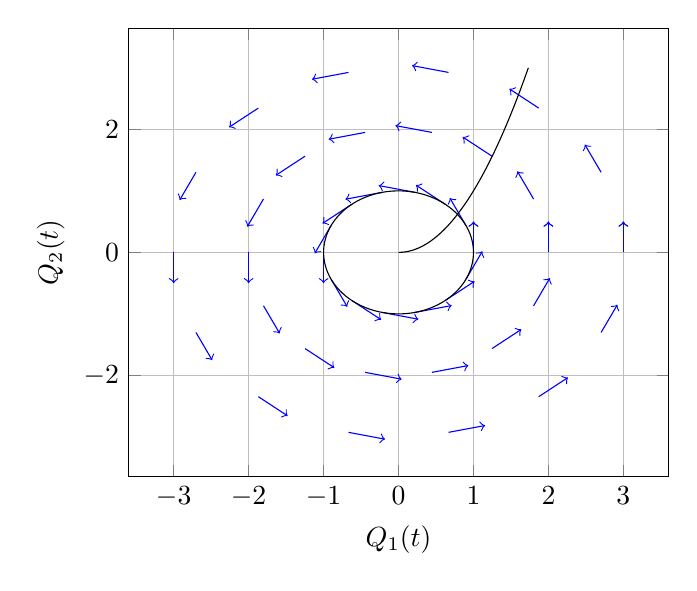
\begin{tikzpicture} 
\begin{axis}[grid=major,xlabel=$Q_1(t)$,
  ylabel=$Q_2(t)$] 
\addplot[samples=15, domain=0:2*pi, variable=\t,
quiver={u={-sin(deg(t))}, v={cos(deg(t))}, scale arrows=0.5}, 
  ->,blue]({cos(deg(t))}, {sin(deg(t))});  
\addplot[samples=15, domain=0:2*pi, variable=\t,
quiver={u={-sin(deg(t))}, v={cos(deg(t))}, scale arrows=0.5}, 
  ->,blue]({2*cos(deg(t))}, {2*sin(deg(t))});  
\addplot[samples=15, domain=0:2*pi, variable=\t,
quiver={u={-sin(deg(t))}, v={cos(deg(t))}, scale arrows=0.5}, 
  ->,blue]({3*cos(deg(t))}, {3*sin(deg(t))});  
\addplot[samples=100, domain=0:2*pi] ({cos(deg(x))},{sin(deg(x))}); 
\addplot[samples=100, domain=0:sqrt(3)] ({x},{x^2}); 
\end{axis}
\end{tikzpicture}  
% \end{center}
\end{figure}
Now, it is easy to check the corresponding invariance condition first
introduced in (\ref{SimpleCDC}). Let $G_z(z)$ denote the Frechet
derivative (which in turns is the Jacobian in this deterministic and
finite-dimensional case) of $G$ at $z$. The columns of the matrix
representation of $G_z$ are the tangent vectors above
(\ref{SimpleCDC}), so the tangent space $T_q(\mathcal{S}^1)$ to
$\mathcal{S}^1$ at $q=G(z)$ coincides with the image $Im[G_z(z)]$:
$$
G_z(z)=[ -\sin(z) \;\cos(z) ]^T.
$$
Recall that the vector field $\mu$ at $q=G(z)$ is in turns:
$$
\mu(G(z))=[ -\sin(z) \;\cos(z) ]^T.
$$
We thus trivially have
$$
\mu(G(z)) \in Im[ G_z(z)],
$$
and, in fact, this is the consistency condition we have to check out
for pairs ($\mathcal{M}$,$\mathcal{G}$) when $\mathcal{M}$ is an
autonomous and deterministic differential system of finite dimension.
\newpage\mbox{}\thispagestyle{empty}

